\documentclass{acmtog}
\usepackage{amsmath}
\usepackage{float}
\usepackage[utf8]{inputenc}
\usepackage{graphicx}
\usepackage{hyperref}
\usepackage[flushleft]{threeparttable}
\acmVolume{1}
\acmNumber{1}
\acmYear{2016}
\acmMonth{June}
\acmArticleNum{1}
%\doi{10.1145/1559755.1559763}


\begin{document}
\makeatletter
\def\runningfoot{\def\@runningfoot{}}
\def\firstfoot{\def\@firstfoot{}}
\makeatother



\title{Algorithms for the automatic layout of multiple windows: \\Practical implementations for Tide}

\author{Nataniel Hofer, supervised by Raphaël Dumusc, Stefan Eilemann and Pr. Felix Schürmann \\
At Ecole Polytechnique Fédérale de Lausanne\\
Neurocomputing semester project}

\maketitle
\begin{abstract}
The present paper focuses on the problem of automatic layout of multiple windows. We consider two different approaches. The first one is to bring the problem to a known global optimization program. The second method used consists at finding an heuristic algorithm which optimizes the visual result in multiple steps. 
\end{abstract}

\section{Introduction}
Tide is a user-interface project for running large display on multi-screen. At Campus Biotech, in the Blue Brain Project (BBP) premises, there are three display wall. Two of them are composed of 4x3 screens of 1920x1080 pixels. The other one is 3x3. Tide is distributed and runs on any number of machines. It is the only open-source software for touch screen which scales to any size of display. At BBP it is mainly used for scientific collaboration since it allows for more interactive presentations  than powerpoints. The display wall allows  high-resolution content, it enables pdf and movie support, and has a desktop streaming feature. With the impeding arrival of an open-deck, 
%TODO ask raphael the specificities of display walls
a 3D stereo feature has been added to improve immersiveness. \\
Tide runs three different display mode:\\
-Default: where you can select windows, resize them and move them around \\
-Fullscreen: where the selected image will occupy most of the space available while keeping its ratio; \\
-Focused: where  all the selected images are displayed on one line according to the order on default mode, projecting them to the foreground. The image are then resized to keep their original ratio;\\
The presented work focuses on the later. 
The previous algorithm was unsatisfying when more than a few windows were displayed, because most of the space was unused. The single line display forced a small height on the windows, thus making the content difficult to see.  \\
This papers explores various algorithms with different approaches to address the automatic layout problem.\\


\section{Modelizing the problem and related work}

As previously stated, the ancient algorithm was unsatisfying, because of the visibility of the content and the usage of available space. We must find all characteristics  an algorithm should have for this task to be satisfying. The answer is not trivial as multiple criterions must be taken into account. Some of those criteria  may not be easy to describe mathematically. However there are three constant rules : the original ratio must be preserved, all the windows should fit on the screen and windows must not overlap. Those constraints are easy to satisfy and formulate.\\
The problem itself is not clearly defined. We would like the result to be ``pleasing to the human eye" or close to what a human may do manually. But the human evaluation of the visual aspect is subjective and hard to expain to a computer. We avoid complications by splitting the visual aspect into subcriteria:\\
%TODO see if bullets are better
-The windows are regularly spaced \\
-Windows do not overlap \\
-Unused space is minimal\\
-Variance in area is minimal\\
Multiple ways to tackle this problem will be discussed, each one having pros and cons. Most of them will lack analysis of result since implementation time was limited. 

\subsection{As a classical optimization problem}

\subsubsection{Finding a feasible solution}
We denote $l_i$, $r_i$, $t_i$, $b_i$, being respectively the coordinates of\,: the left edge, the right edge, the top edge and the bottom edge of the $i^{th}$ window (x axis grows right, y axis grows down, origin point(0,0) is set at the topleft corner of the screen ). Those are our output variables. Our input values are\,:  $W$ and $H$, the width and the height of the available space, n the number of windows and $R_i$ the ratio of the $i_{th}$ window. Then we can write the former constraints as\,:

\begin{equation}
\dfrac{r_i - l_i}{b_i - t_i} = R_i \quad \forall  i \in  \{1, ... n\}
\end{equation}

\begin{equation}
\begin{split}
&\forall  i \in  \{1, ... ,n\}  :\\
&l_i \geq 0 \wedge t_i \geq 0 \\
&r_i < W \\
&b_i  < H  \\
&l_i < r_i \wedge t_i < b_i
\end{split}
\end{equation}


\begin{equation}
\begin{split}
&\forall i, j \in \{1,..., n\}, i < j : \\
&(t_i > b_j) \lor (b_i < t_j) \lor (l_i > r_j) \lor (r_i < l_j)
\end{split}
\label{eq:logical}
\end{equation}

\subsubsection{Tuning an objective function}
A constraint solver can easily find a feasible solution. However this solution may not be satisfying since all the windows may be too small or not centered. What we precisely want is not clear, however we can turn this problem into a quadratic optimization problem with a few tricks. We set the objective function  to :\\
\begin{equation}
f_0(n) = max \sum_{i=1}^{n}{(r_i-l_i)(b_i-t_i)}
\label{eq:objective}
\end{equation}
To get rid of the logical constraint in equation (\ref{eq:logical}), we use the method from \href{https://ocw.mit.edu/courses/sloan-school-of-management/15-053-optimization-methods-in-management-science-spring-2013/lecture-notes/MIT15_053S13_lec11.pdf}{this excellent course of the MIT}.\\ 
We introduce a constant $M$, big enough such that every constraint is satisfied if we put it to the right-hand side of an equality. Then we add binary variables $w_m$, and add to the right handside of the equation either $(1-w_m) M$ or  $w_m(M)$. Thus inequalities in (\ref{eq:logical}) become\,: 

\begin{equation}
\begin{split}
&\forall i, j \in \{1,..., n\}, i < j : \\
&b_j - t_i < w_mM + w_{m+1}M \\
&b_i - t_j < (1-w_m)M + w_{m+1}M \\
&r_j - l_i < w_mM + (1-w_{m+1})M \\
&r_i - l_j < (1-w_m)M + (1-w_{m+1})M\\
\end{split}
\end{equation}

Thus, our problem almost becomes a quadratic programming instance (because of the integer binary variables it is not).
We can bypass this issue by first assigning the binary variables and then solving the quadratic programming problem using Lagrange multipliers.  %TODO cite Frank, Marguerite and Wolfe, Philip -> bibtex
%TODO reminder of big O notation ?
Complexity explodes since there are $O(n^2)$ variables, so $O(2^{n^2})$ assignments possible. In practice, for Tide, n would rarely exceed 20. Hence brute force may be a viable solution. If computation is slow, assigning randomly those variable and solving the quadratic program may be a better alternative. \\
At this point, we are guaranteed to have a satisfying occupancy of the space. But we still have the issue that windows can have close to 0 width. There are two possible workaround : \\
-Add constraints to enforce a min size for the windows; \\%trade of, computationnally expensive bigger constraint
-Add a penalizing term to the objective function. \\
Depending on the min size constraint, the first alternative  may lead to an empty feasible set. Running the algorithm for different values of min size will lead to a satisfiable solution, with an increase in computational cost. \\
The difficulty in the second alternative is to find a function which penalizes smallest and biggest windows. We suggest to add to the objective function (\ref{eq:objective}) the following term :
\begin{equation}
\lambda \sum_{i = 1}^{n}{w_i + h_i}
\end{equation}
 Where $w_i = r_i - l_i$ and $h_i = t_i - b_i$ and $\lambda$ is a real that must be tuned appropriately. \\
Our algorithm has improved but is still unsatisfying since there is no guarantee of equilibrium. %TODO think of an example
Similar input conditions may lead to very different results. Implementation of this algorithm has been put aside to the profit of more heuristic ones, allowing for a greater control over the output.


\section{Heuristic algorithm}

\subsection{Introduction}

Since we convinced ourselves that an optimal solution may be hard to compute, we looked for an algorithm which gave good results in most of the cases without any ``hard" guarantees

\subsubsection{Main principles}

. The idea is to construct a rectangle containing all the windows with ratio as close as possible to the available space. We start with an empty tree and add all the windows one by one. Once there is no remaining window, we resize the tree to fit in the available space. For this algorithm to perform well, we need to keep a rootNode whose surface is similar to the available space (meaning their ratio width/height are close). 

Any node in this tree is a rectangle composed of two children which are contiguous. A leaf that contains a window is called ``full" and a leaf that does not contain a window is ``empty".  \\
%TODO add scheme for horizontal or vertical cuts

The insert procedure is easy to implement. We try inserting recursively in the tree, searching for a big enough empty leaf . If such insert is unsucessful, we create a new rootNode containing the new window and the previous tree as children. The position of the new window is chosen so the tree is closest to the objective ratio. (see Figure \ref{fig:SimpleInsert}, \ref{fig:Insertion} and \ref{fig:InsertionFin} for an example)

\begin{figure}
  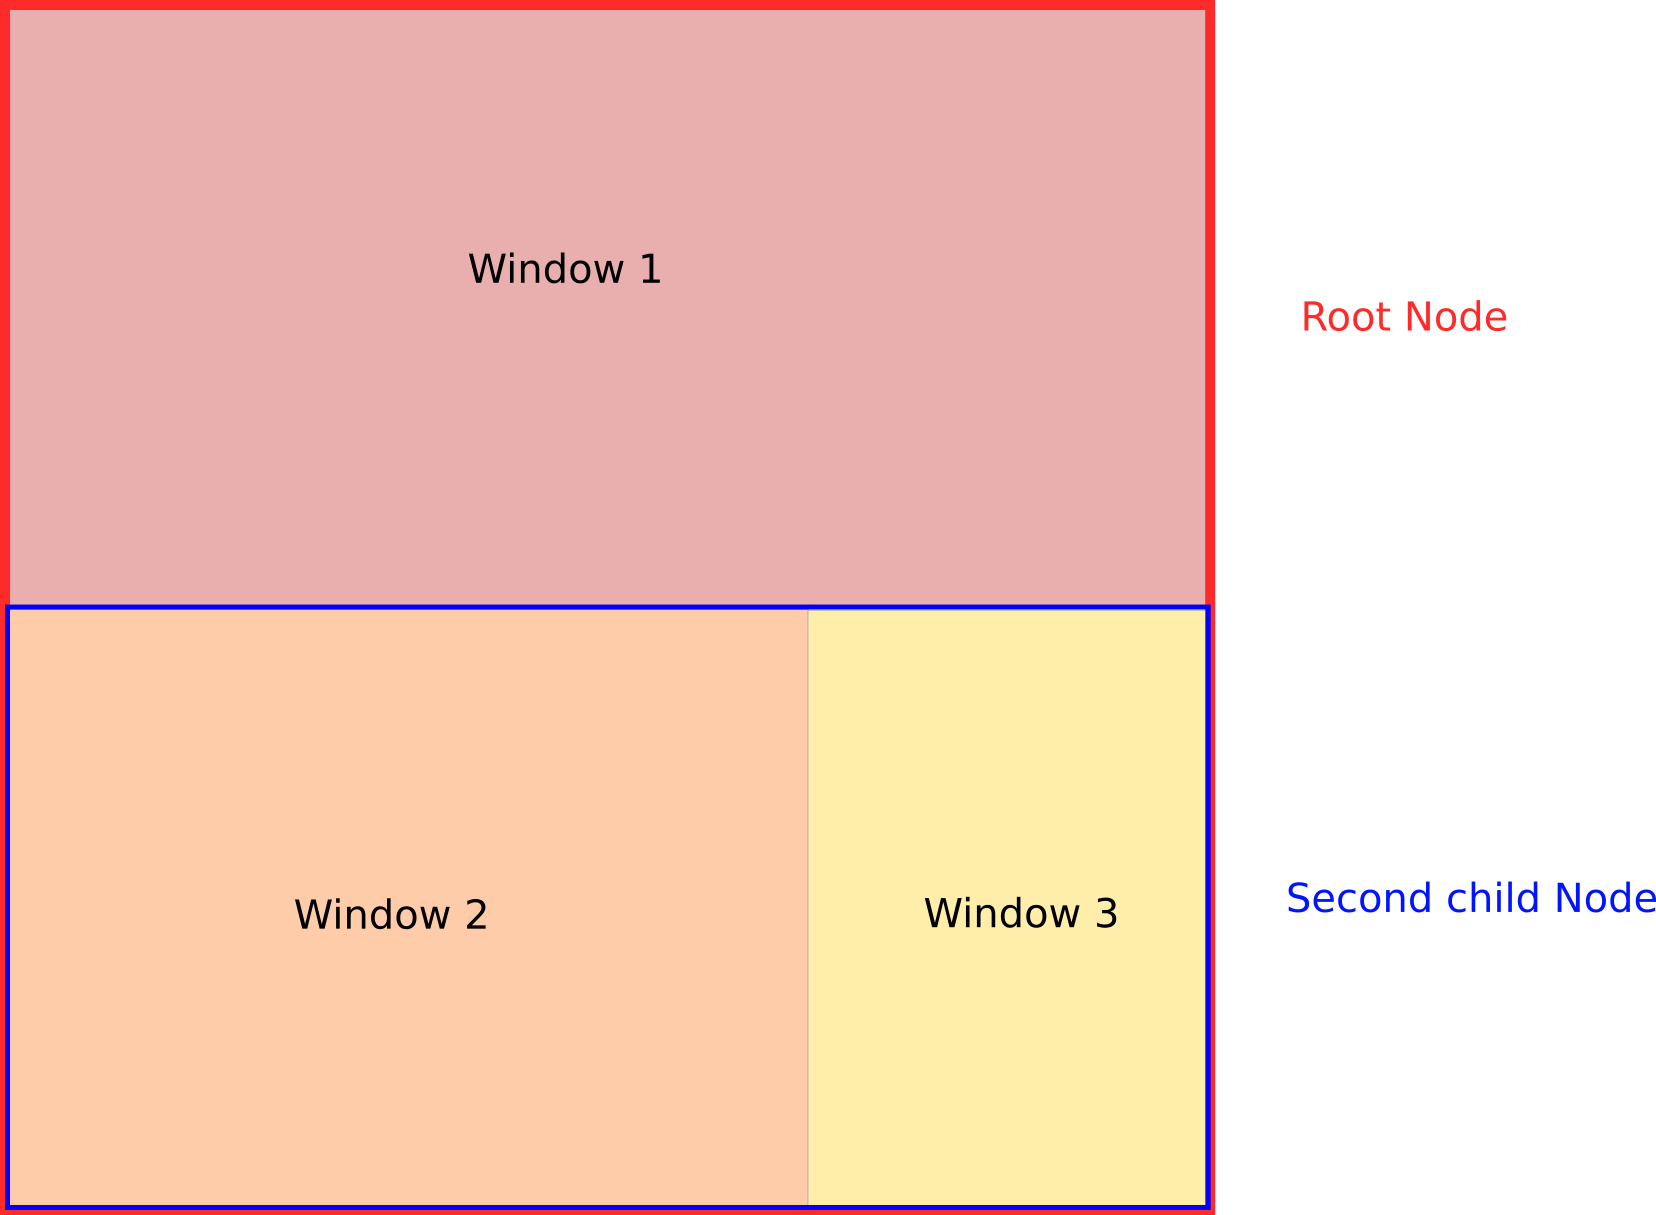
\includegraphics[width=\linewidth]{Images/1erDessin.png}
  \caption{Insertion of 3 windows into an available space of ratio 1}
  \label{fig:SimpleInsert}
\end{figure}

\begin{figure}
  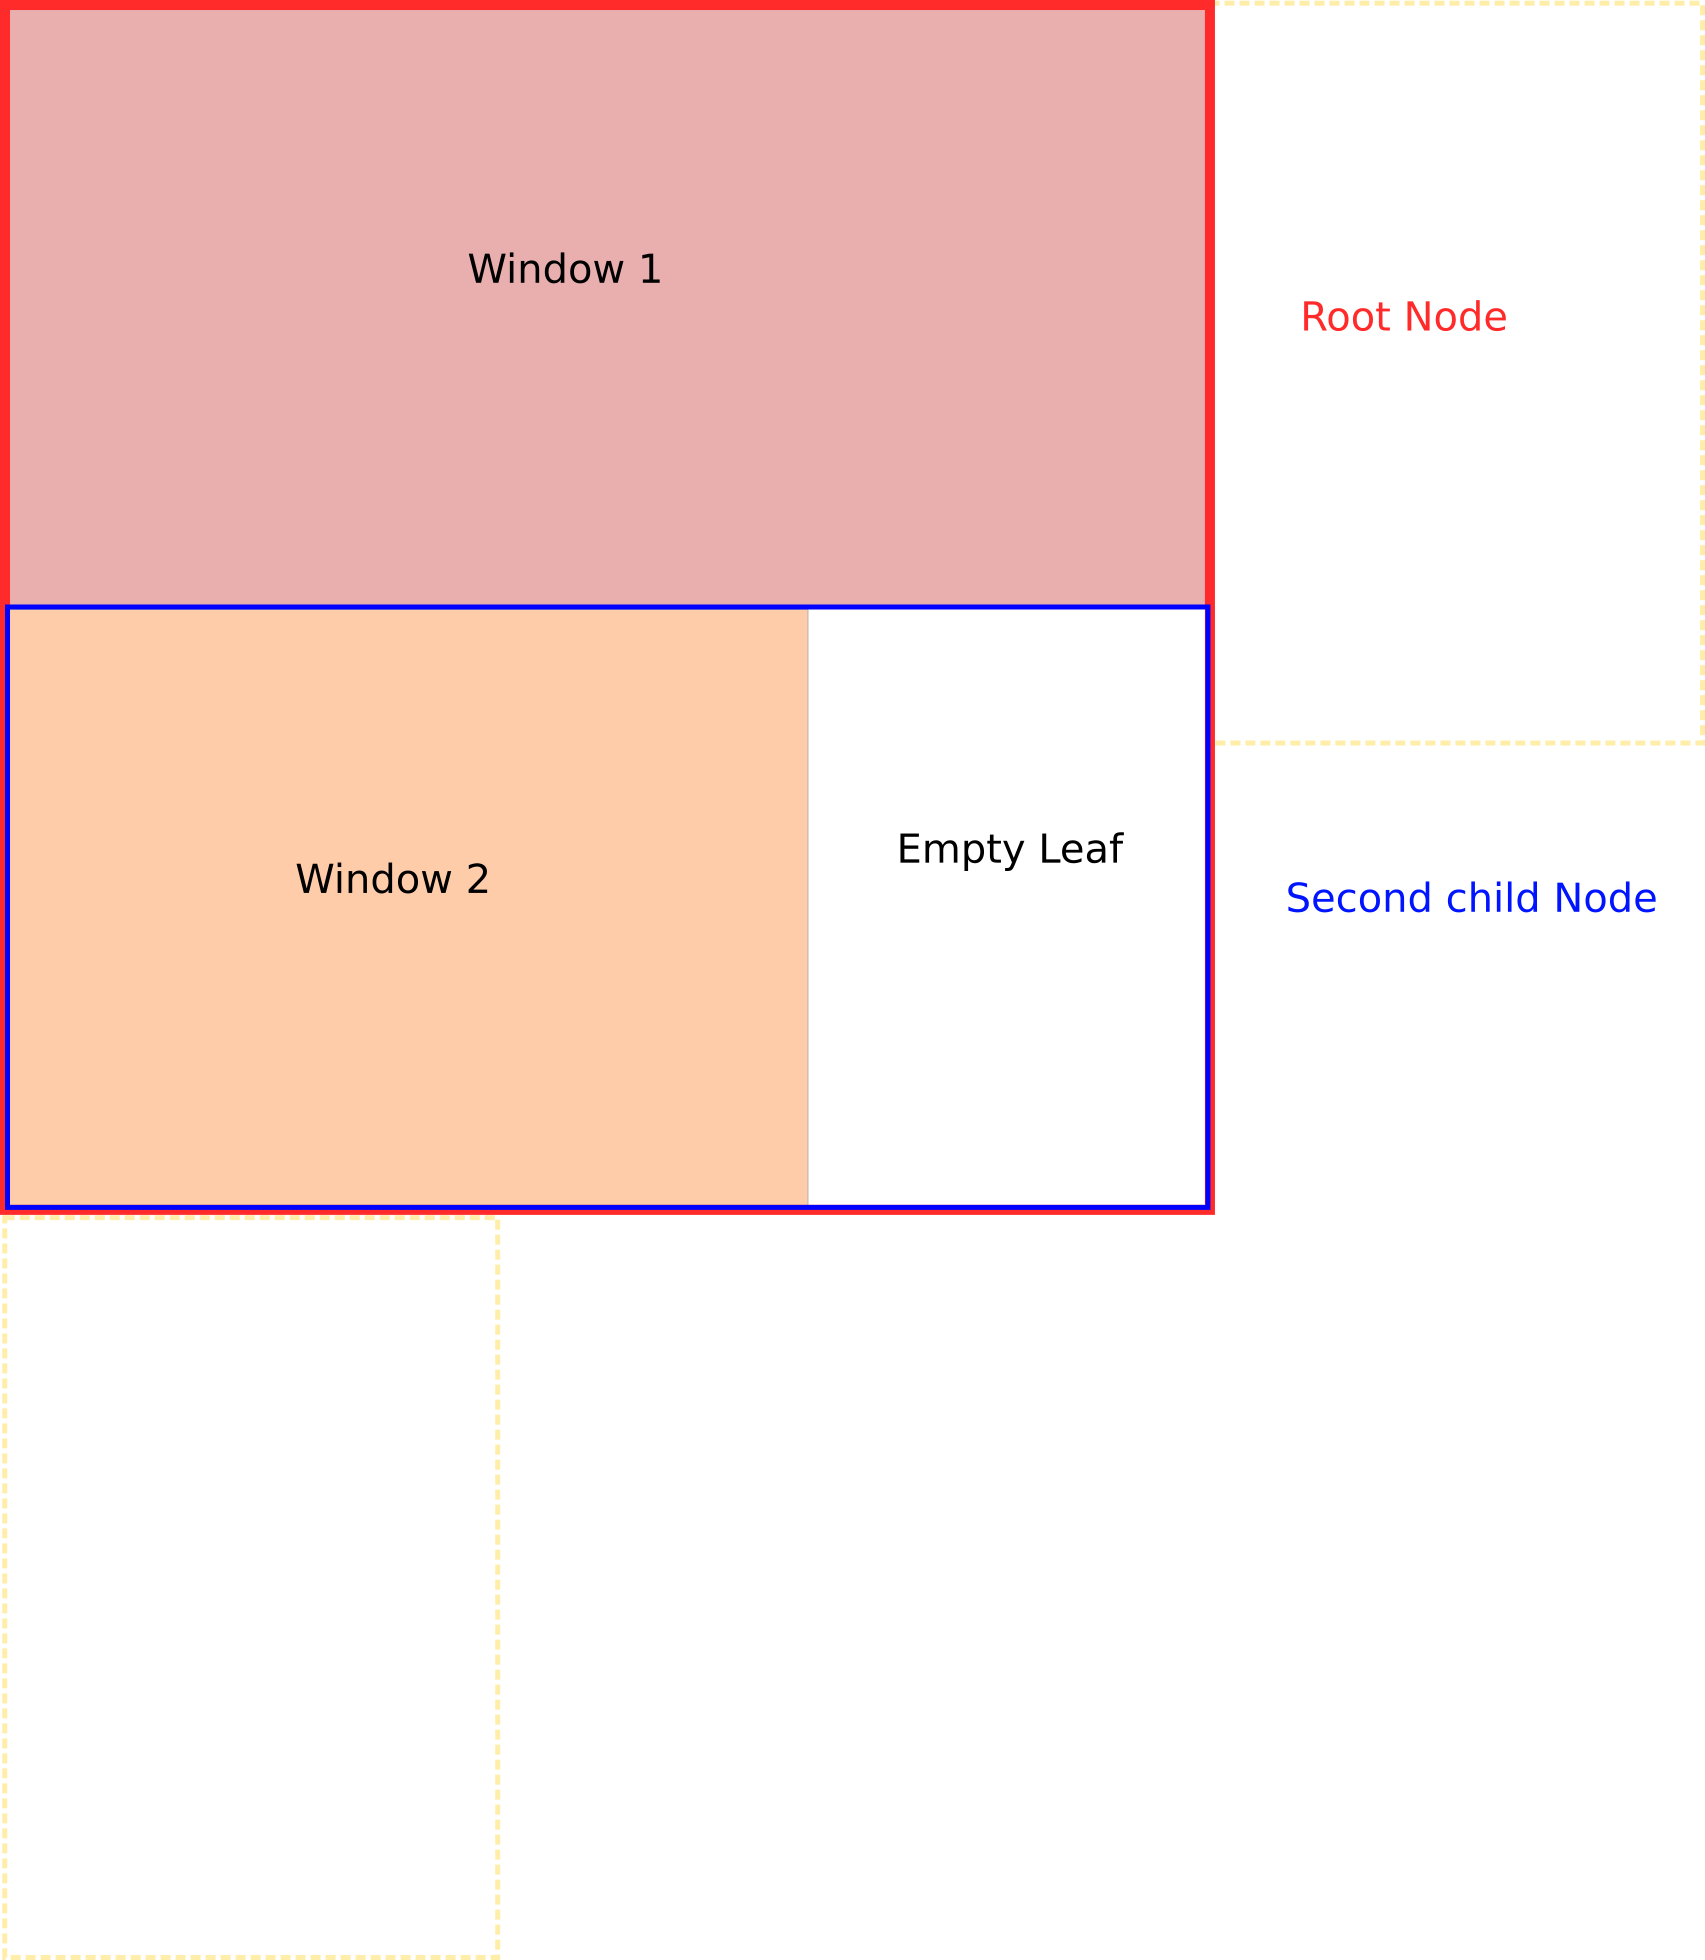
\includegraphics[width=\linewidth]{Images/Insertion.png}
  \caption{This time the empty leaf is too small, we choose emplacement to the right because of the ratio = 1}
  \label{fig:Insertion}
\end{figure}

\begin{figure}
  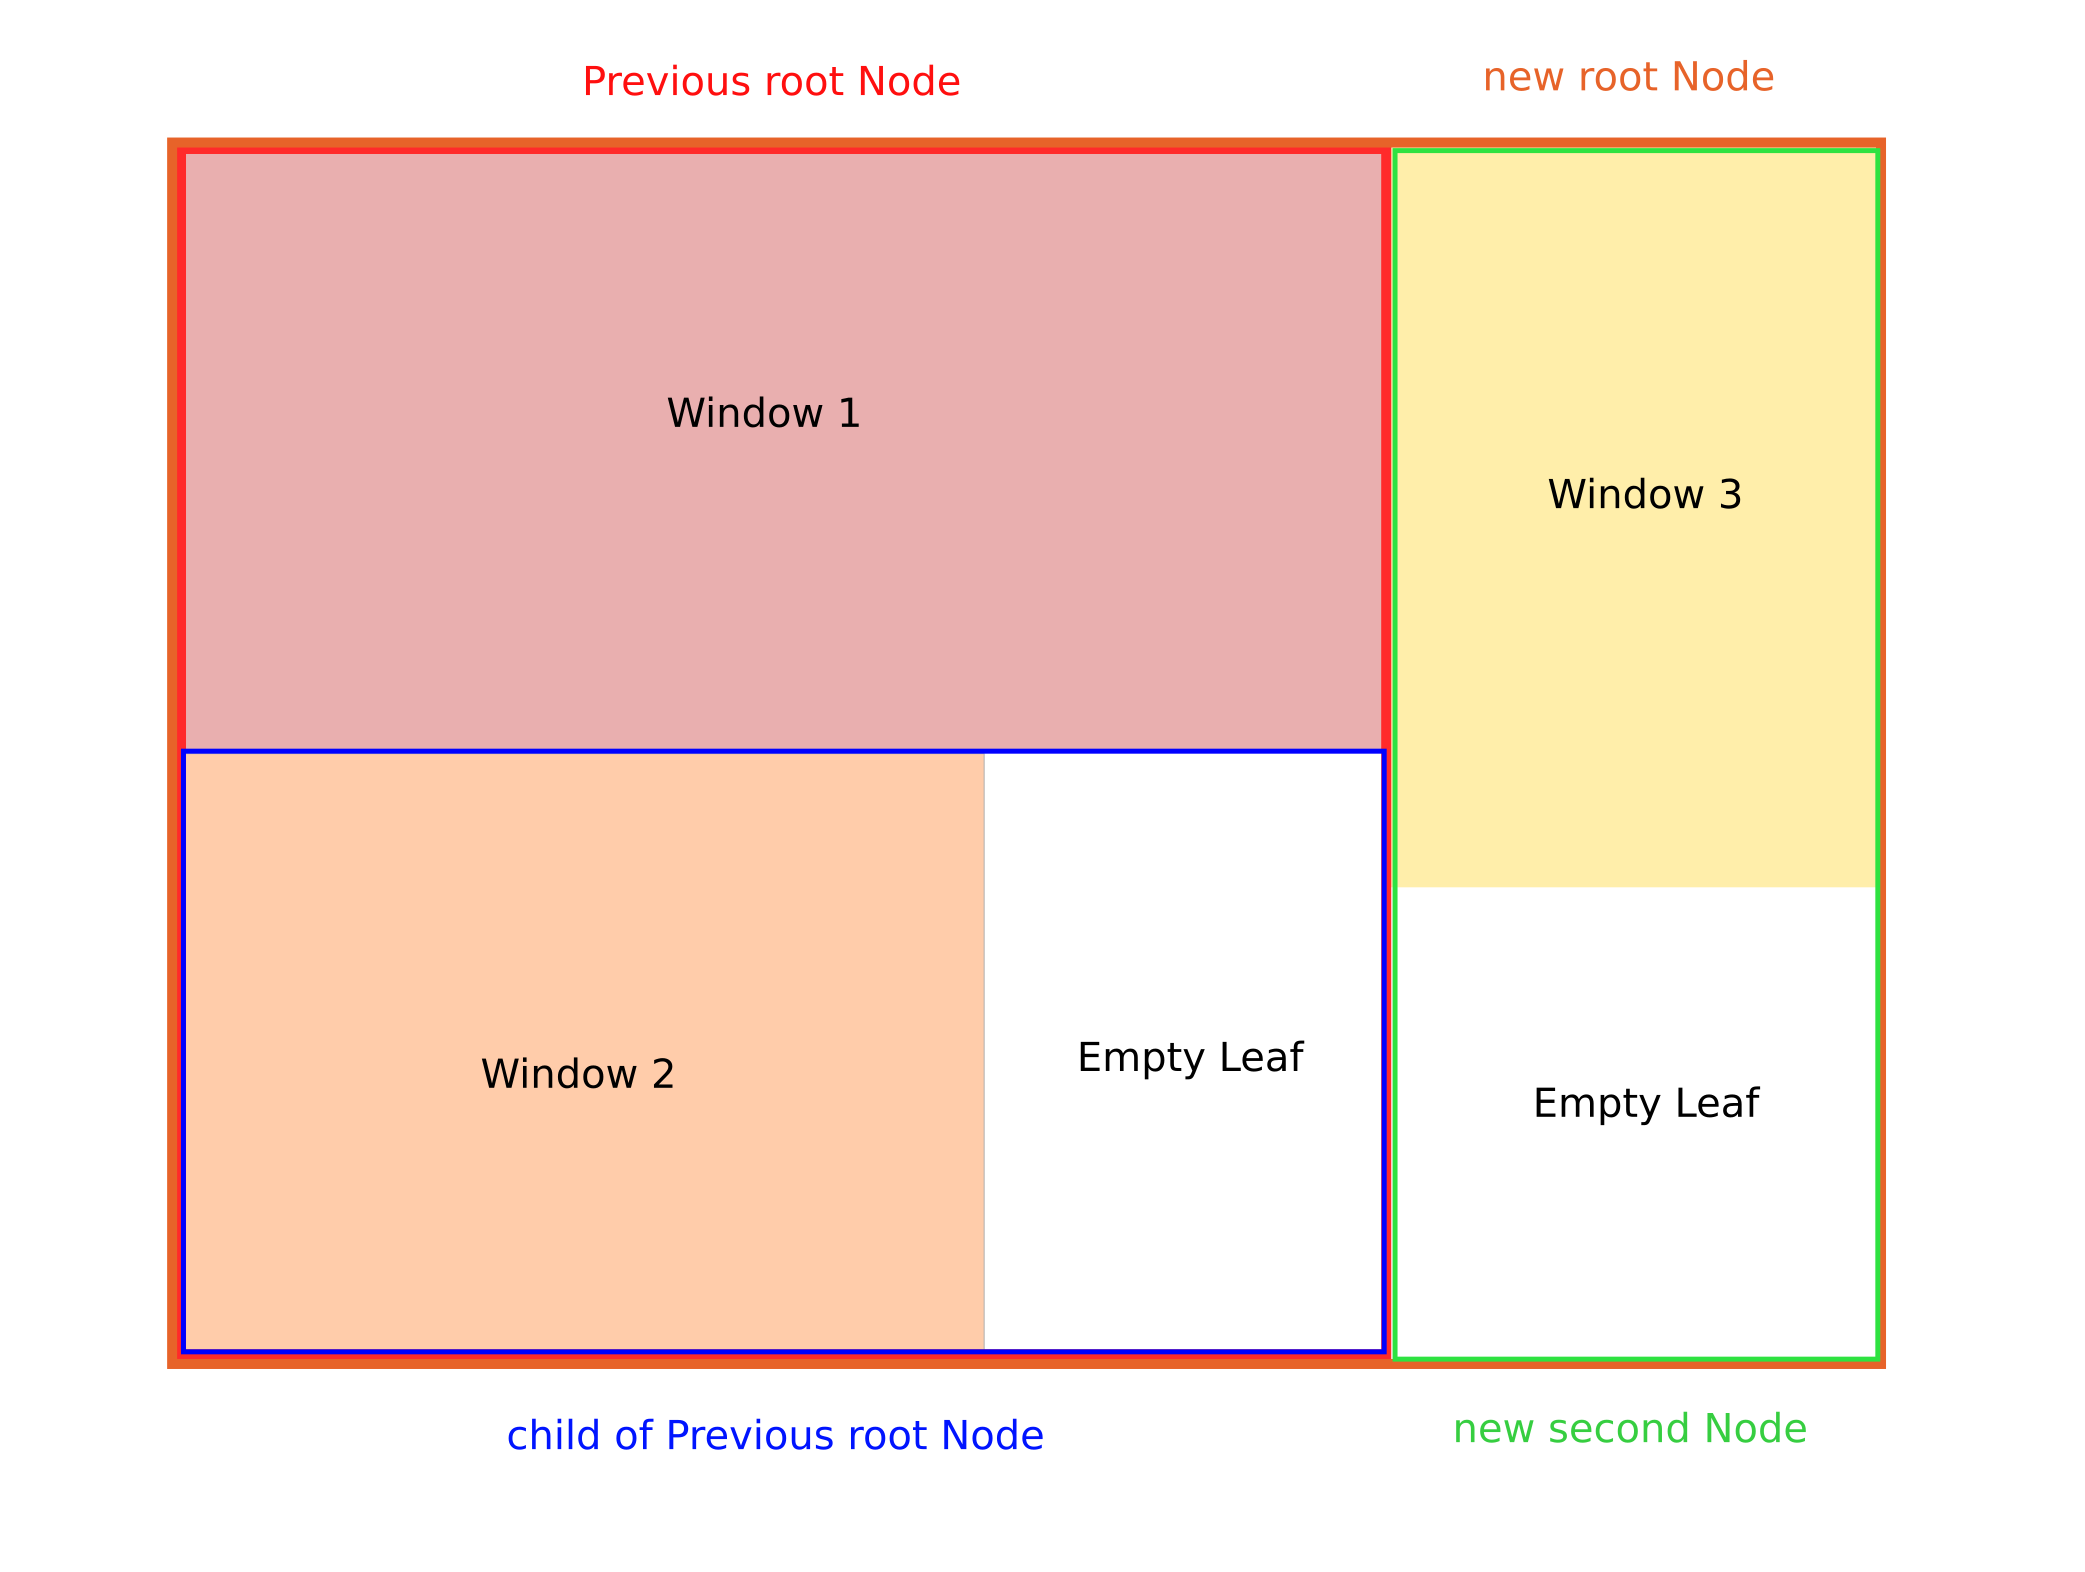
\includegraphics[width=\linewidth]{Images/InsertionFin.png}
  \caption{The structure of the tree has been changed}
  \label{fig:InsertionFin}
\end{figure}

\begin{figure}
  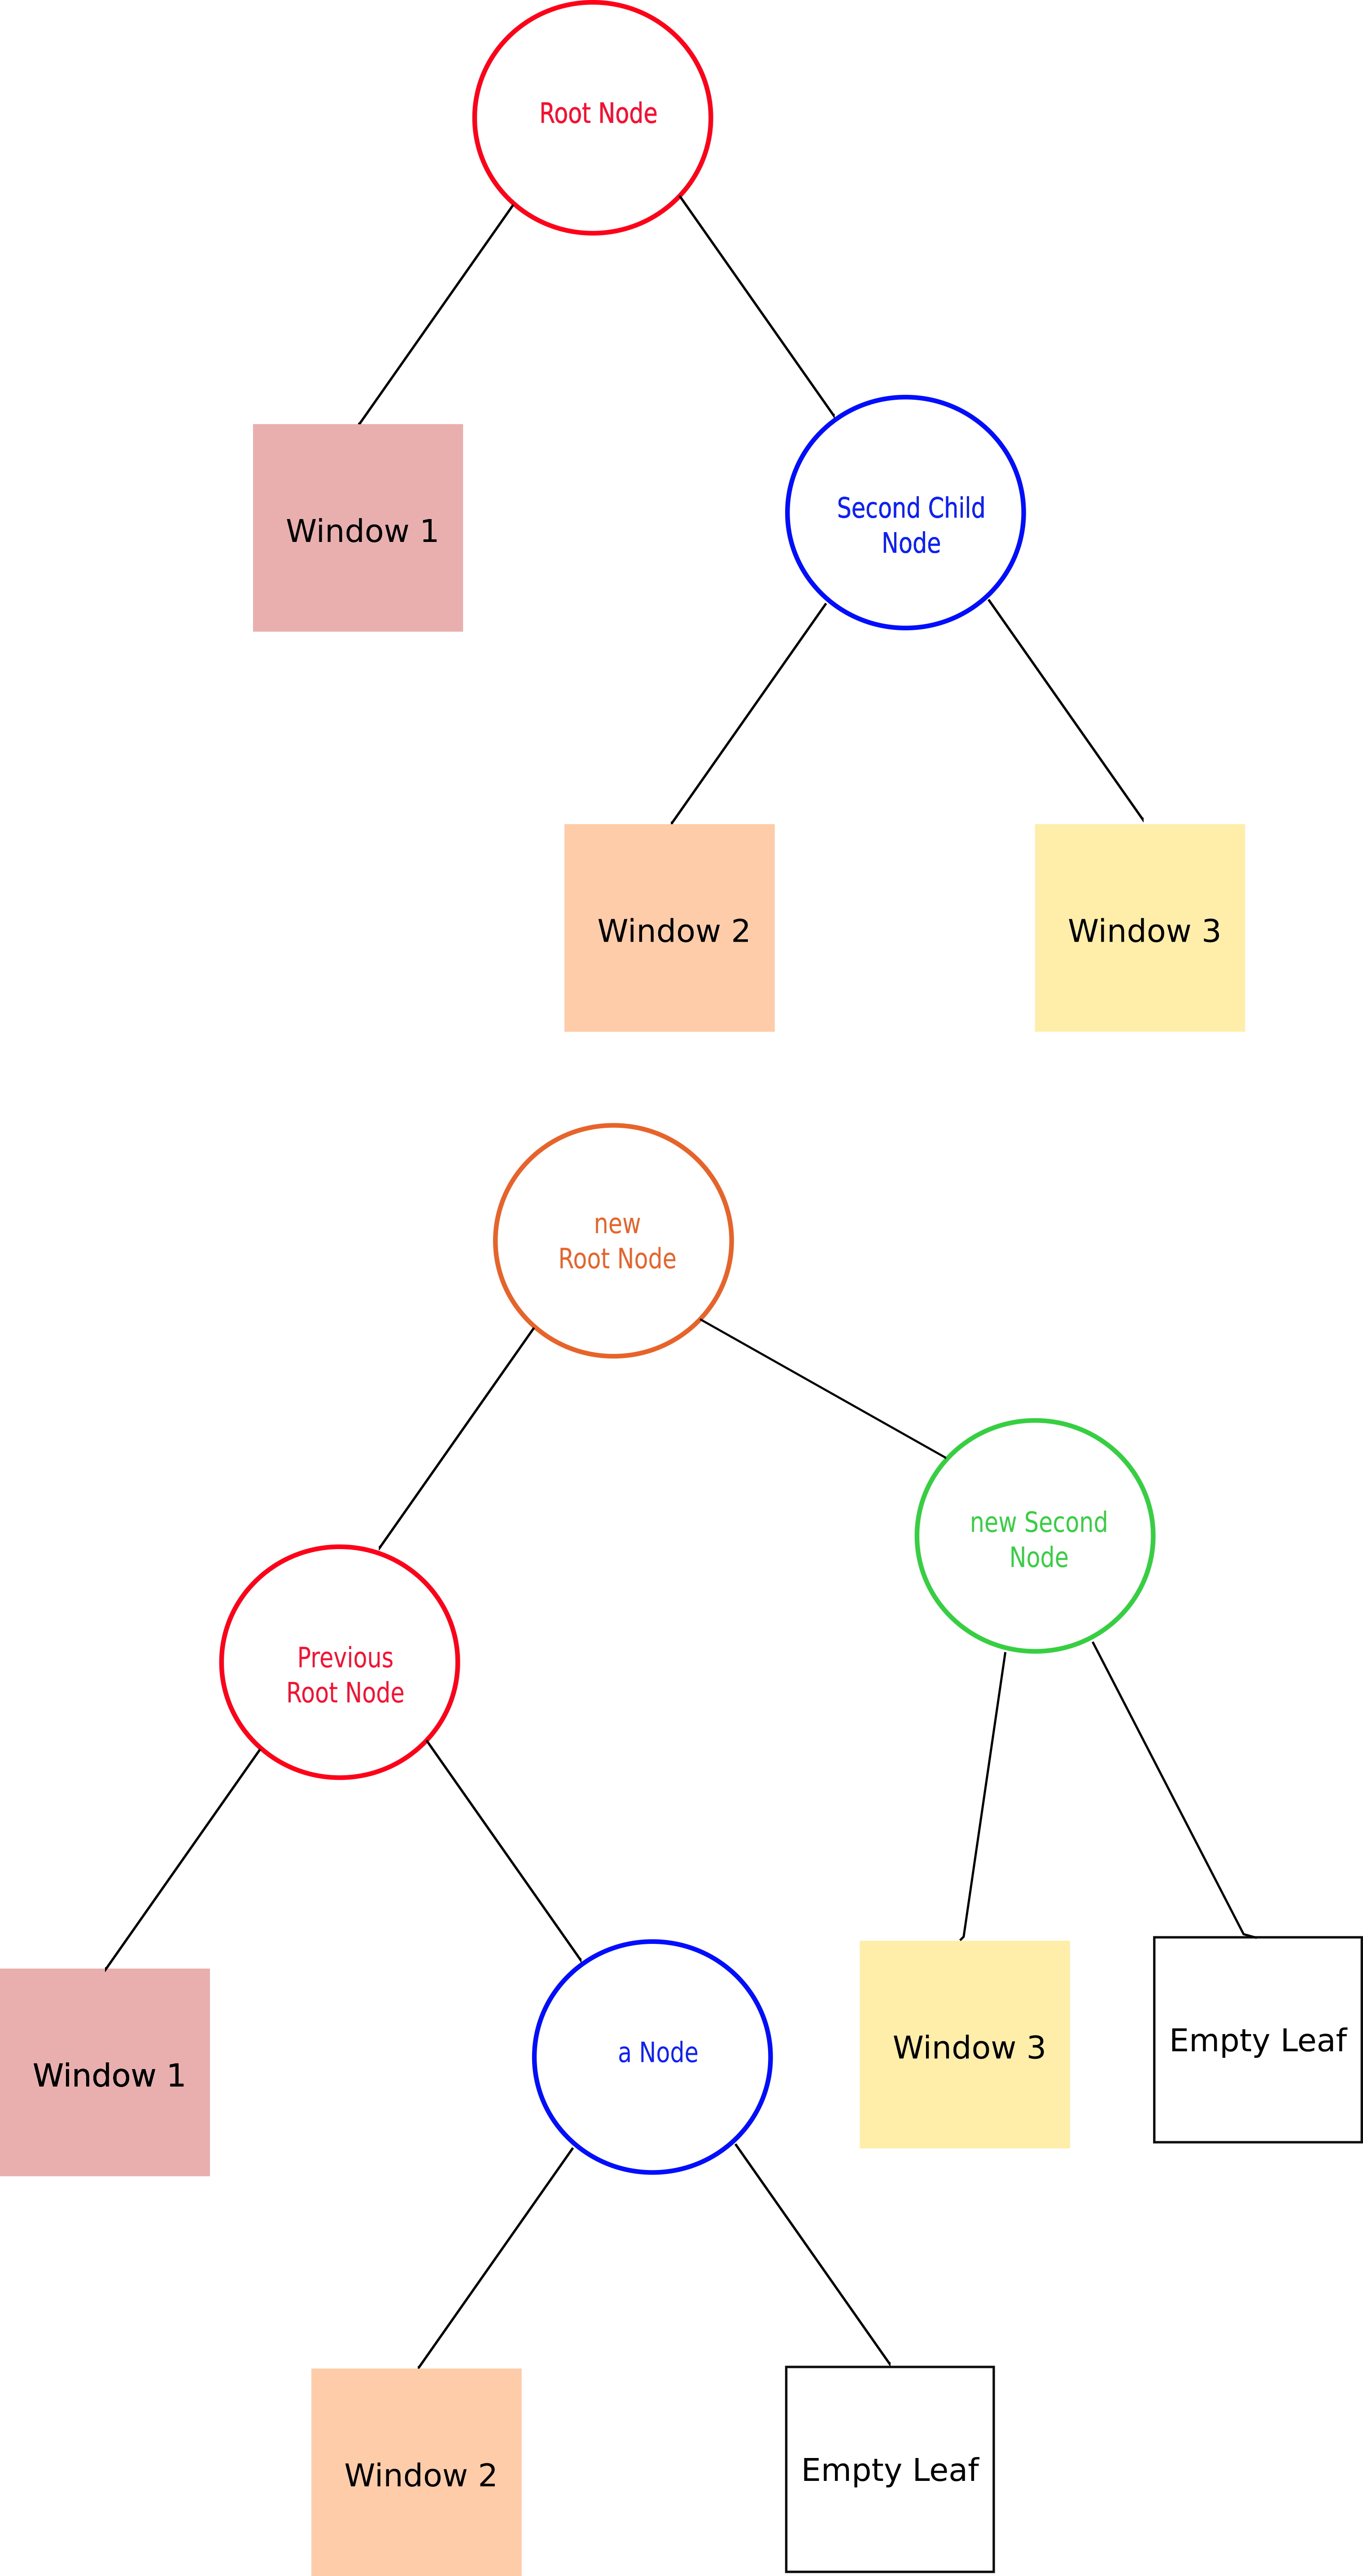
\includegraphics[width=\linewidth]{Images/Treestructure.png}
  \caption{comparison between the tree structure of Figure \ref{fig:SimpleInsert} (top) and Figure \ref{fig:InsertionFin} (bottom)}
  \label{fig:TreeStructure}
\end{figure}

Once the inserting part is done, our tree (or rootNode since it is equivalent) may be way bigger than our available space. Or, on the contrary, very small. This does not matter since we resize our tree to fit in the available space. This constraining phase is also easy to implement recursively on our tree, since each node is a rectangle whose space is the sum of its children. When leaves are constrained in a rectangle, they take the biggest space possible without changing their original ratio and are then centered. 

\subsubsection{Initialization choices}

The attentive reader may have noted two unspoken initialization processes which affect the execution of the algorithm. We did not discuss the initial size of the windows and the order in which the algorithm inserts them. \\
In Default mode of Tide, windows have a default size when they are opened (depending on their content). The choice has been made to use this size as the initial size of the windows. By the way the algorithm works, the relative size of two windows on the focused mode is the same than in Default mode. This is a benefit in most of the cases, where windows in Default mode are already balanced. But it leads to degenerate cases when a window occupies the majority of the screen in Default mode. Such cases can be detected and an initial resizing of the window may occur. An other benefit resulting from this initialization is the control over the algorithm brought to the user. He can decide on Default mode to increase the size of a window and this will impact its size in focused mode. At the moment it is the only control the user has on the display of this algorithm. In the previous focus mode, control offered to the user laid in the order (left from right) of the windows. \\
This is not the case anymore with this algorithm since the order of the windows depends on the maximum of their relative width or relative height compared to the available space. Those ``bigger" windows may indeed prove troublesome if they arrive last since they are more susceptible to change the ratio of the tree. However, in some cases this ordering is far from the best one. We will see a way to deal with this issue.

\subsection{Issues and workarounds in the algorithm}

 \subsubsection{Representation of empty spaces}
One of the main weakness in the algorithm lies in the representation of empty spaces. A window may fail to insert into two contiguous empty spaces because they lie far from each other in the binary tree representation. \\
%TODO show an example
This issue is the most troublesome for this algorithm as it is intrinsically connected with the binary tree representation which is a key feature for the resizing part. We could imagine a way to detect close empty spaces and considering them as one big empty space, making some insertion to rebalance the tree. This feature has not been implemented yet because it would lead to fundamental changes in the algorithm. We attempted to  address this problem by changing the underlying data structure from a binary tree to a grid of cuts where each window is defined by four cuts, two by two parallel. The insertion part led to better results before the resizing, however the resizing part was far from trivial and may be as difficult as the initial problem. Thus, the idea of cuts has been put aside.
%TODO show a scheme of cuts

\subsubsection{Tolerance factor}
Another flaw is the lack of flexibility when we insert a new window, as we can see in the Figure \ref{fig:Equalbuggy} where four images of the same size are selected. The last image is then inserted to the left instead of having a nice two by two square, due to floating points error. 
\begin{figure*}
  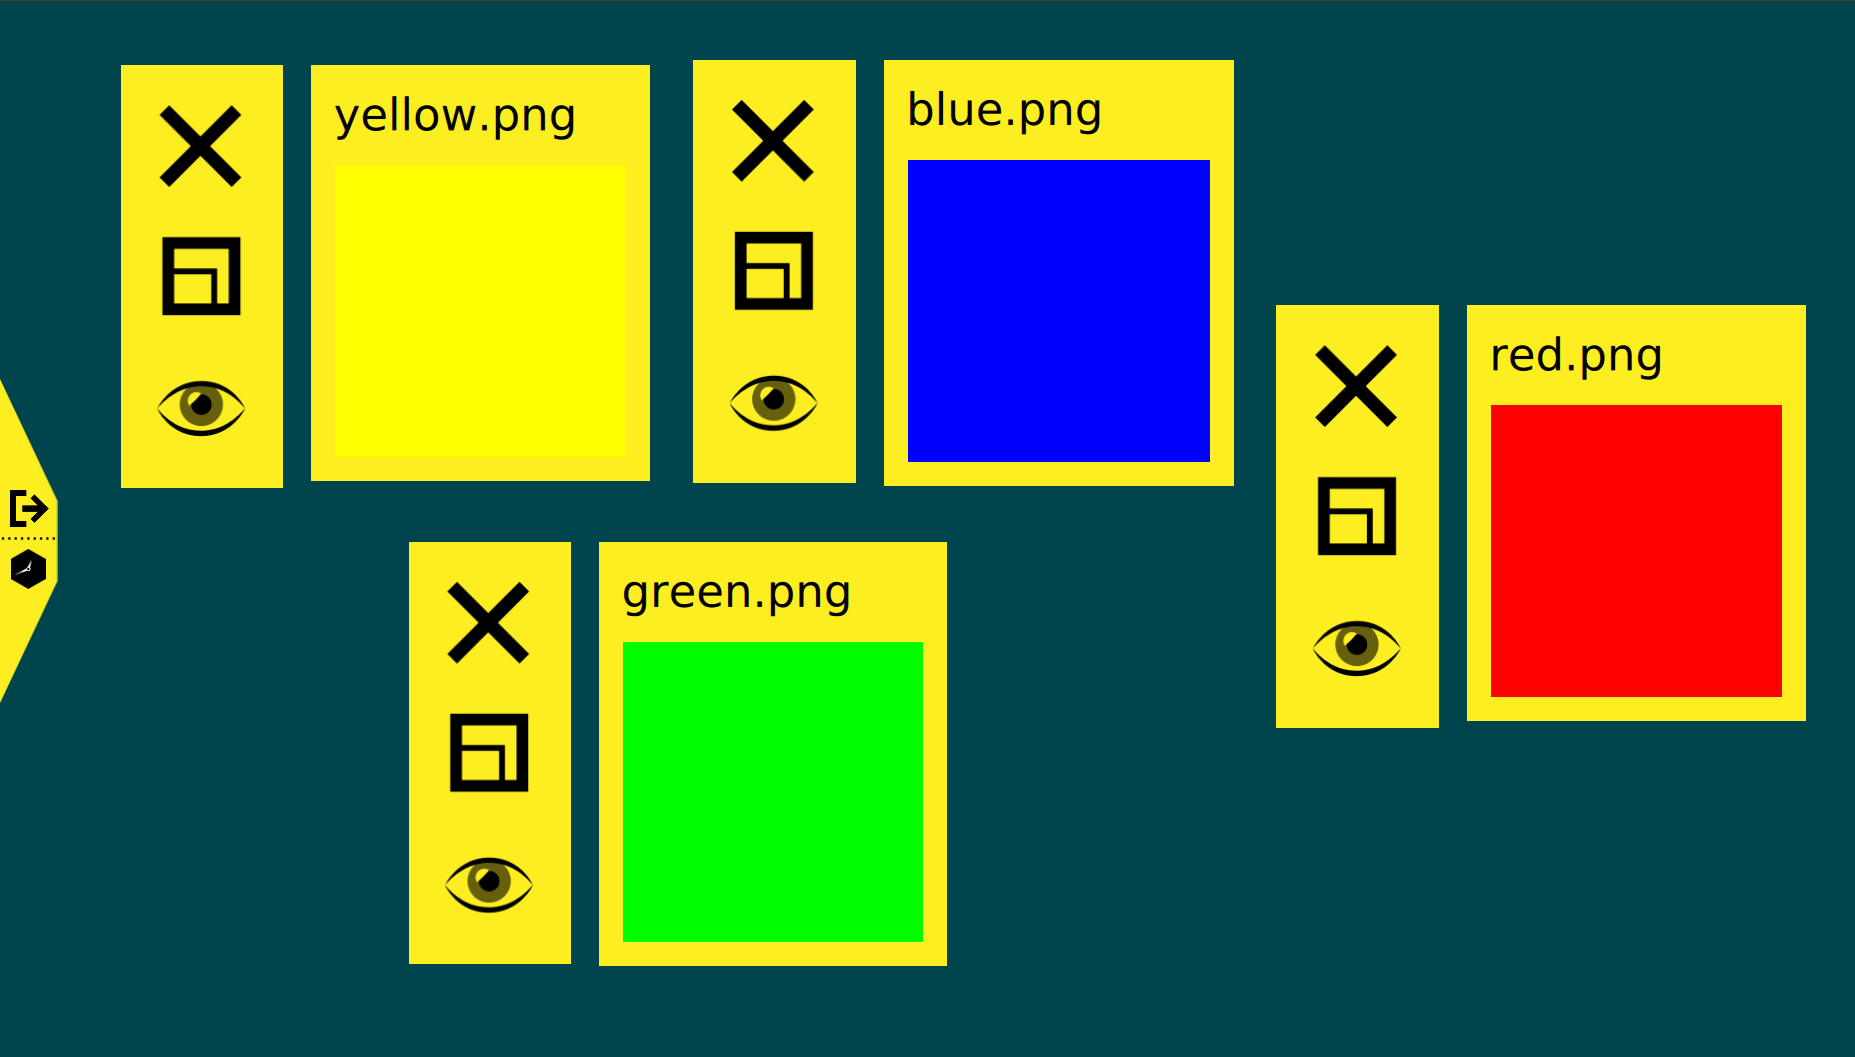
\includegraphics[width=\textwidth]{Images/4-equalbuggyCropped.png}
  \caption{A two by two display here would be nicer}
  \label{fig:Equalbuggy}
\end{figure*}
\\ 
A workaround is to add a tolerance factor when inserting a new window. If the window height and width is no more than 1 + $\alpha$ times the empty space, the window is still added to the empty space, shrinking it if need be. There is a tradeoff for the value of $\alpha$. If it is zero, we lack flexibility as in Figure \ref{fig:Equalbuggy}.
If it is high, the relative size ratio between windows is not respected anymore. Empirically deduced value of $\alpha$ is 0.3. See Figure \ref{fig:Equalright} for an example with tolerance factor.

\begin{figure*}
  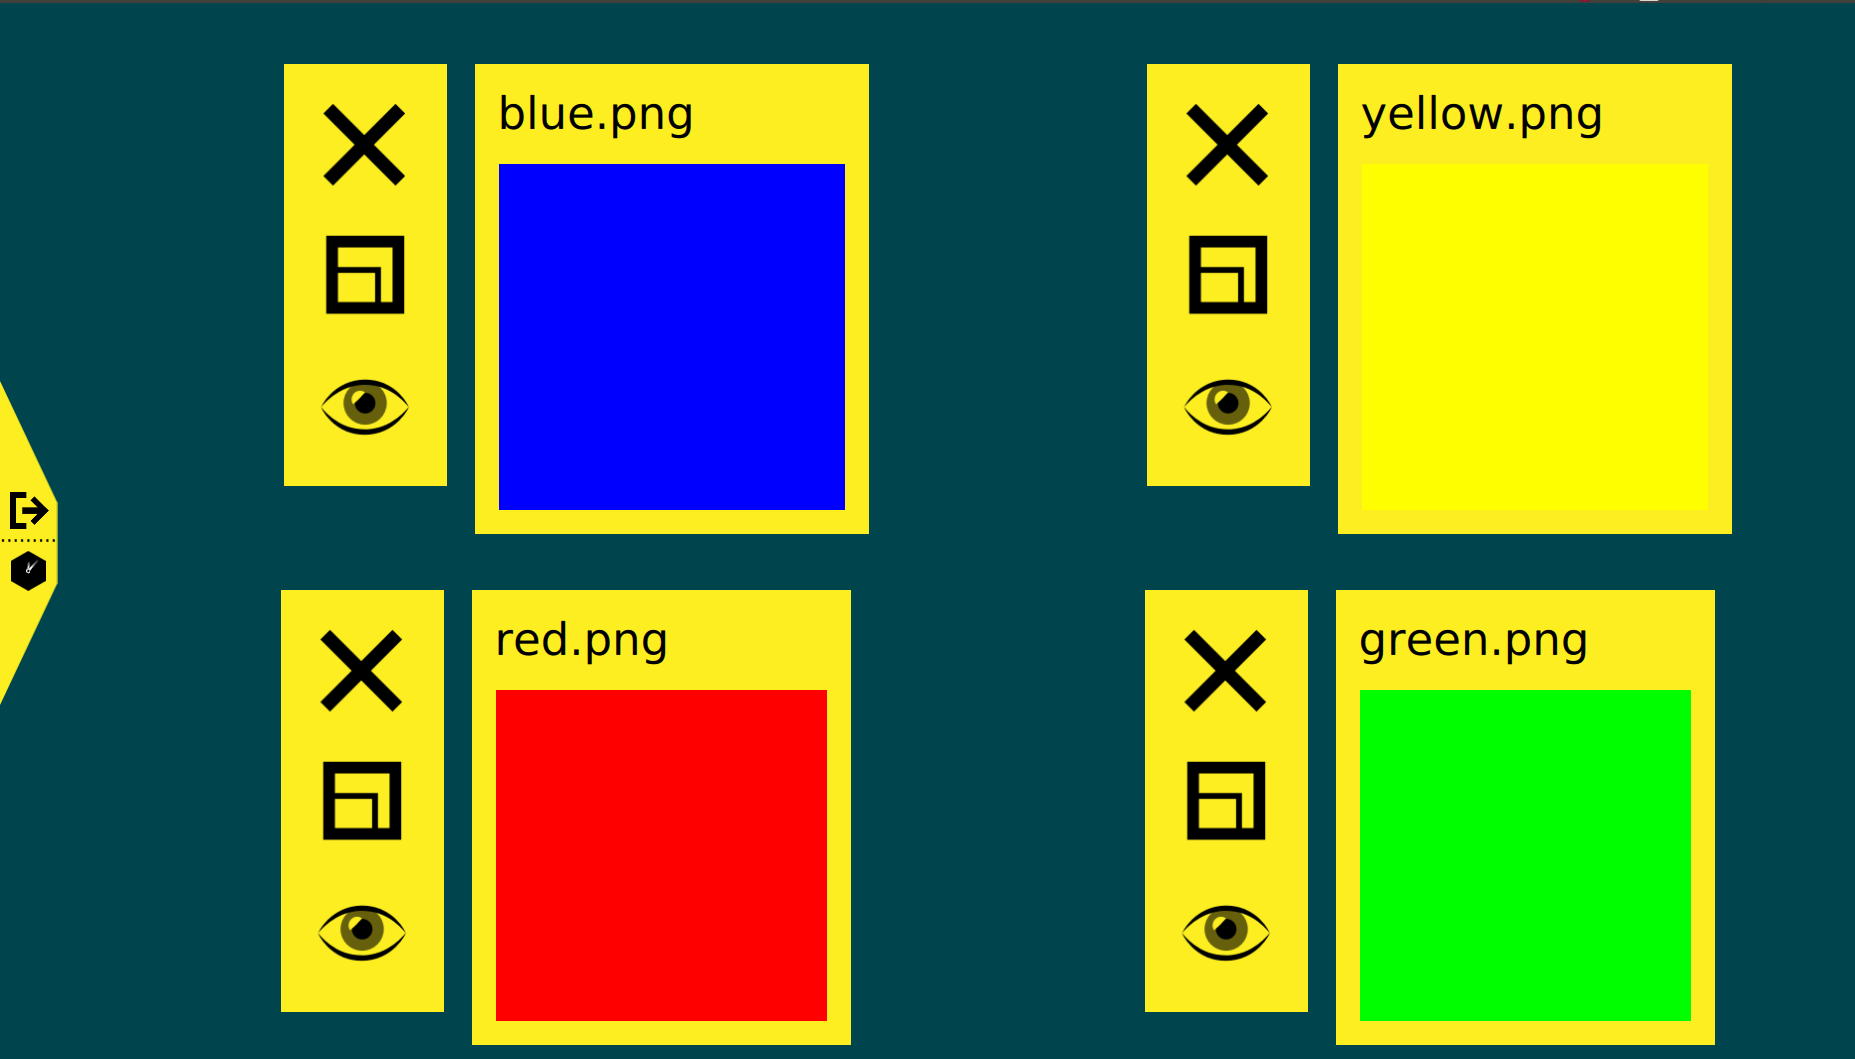
\includegraphics[width=\textwidth]{Images/4-equalToleranceCropped.png}
  \caption{With tolerance factor, we reach a two by two display}
  \label{fig:Equalright}
\end{figure*}

\subsubsection{Order of the windows} While sorting by aspect ratio may often be a good idea, there are always corner cases in which it may be the worst order possible. Such cases arise when a window is big and its ratio is far from the others.
%TODO show an example

A natural way to deal with those cases is to randomize the order of the windows and run the algorithm multiple times, keeping the result for which the occupied space is maximal. Note that brute force requires $O(n!)$ runs and thus is not a viable solution. A specific study of the number of iterations needed to come close to the optimal result has not been established. It has been noticed that this method improved the results compared to the original order. The main issue is that the output is not determined by the input, which can be destabilizing for the user. If the user does not like this, it is always possible to fix the seed of the random function. The same input will always produce the same output, which can be an issue on specific inputs. However there is no reason that someone would ``cook up" especially bad inputs, and thus having a known pseudo-random function instead of an unfathomable one is acceptable.  

\subsubsection{insertion phase using recursivity}
While the improvement randomization brought on the special cases was substantial, the solution it led to was not perfect. The heuristic placement in insertion phase leads to a sparse rectangle. The resizing is then unable to balance the windows in a nice way. Considering each subtree as the same optimization problem with another available space during insertion phase might fix some of those problems. Thus, each node would have a different available space which will not be equal to only the sum of his two childs. According less importance to the rootNode and allowing each node to modify the structure of the tree would add the flexibilty we lack. However this feature has not yet been implemented.

\subsection{Results}

Although the quality of the algorithm was not assessed formally  but more on visual aspects during implementation,  we show here an analysis on different set of windows. Three sets of windows were used. The first one consisted of six windows with high variance in height, width and aspect ratio. The second one had low variance in those parameters while the third one was simply the union of the first two. \\
We used the percentage of space occupied by all the windows relative to the available space as a metric. The previous algorithm along with four different version of the new heuristic one were compared. The first version presented no tolerance factor during insertion and no permutation in the order of insertion of the windows. The second one presented in addition a tolerance factor of 1.3. The third and fourth one had respectively 20 and 200 random shuffles in the insertion order. The results are shown in the Table \ref{tab:results}. \\


\begin{table}[t]
\tabcolsep2pt
\tbl{Percentage of occupied space by windows on different sets}{%
\begin{tabular}{@{}|c|ccc|@{}}\hline

\hline
Algorithm used &Low Variance & High Variance & Mixed\\
 \hline
\hline
Previous algorithm & 9.95 \% & 11.08\% & 2.40\%  \\ 
 \hline
 No tolerance & 61.22\% & 51.81\%  & 51.60\%  \\ 
 \hline
 1.3 tolerance factor & 61.22 \% & 41.94\% & 47.24 \% \\
 \hline
  20 random shuffle &61.89 \%& 69.50\% & 61.88 \% \\
 \hline
 200  random shuffle &63.90 \% & 69.32 \%& 66.50 \%\\
 \hline
\end{tabular}}
\label{tab:results}
\end{table}

The most salient result is the huge improvement in space-using done by the heuristic algorithm over the previous one. Moreover, the algorithm did not lose significant performance even when there was 12 windows (Mixed case). \\
Furthermore, we see that without shuffling the windows, the algorithm performed worse on the high variance set and with shuffling it can find a better solution. In low variance cases, shuffling does not improve much the solution, probably because we are already close to the optimal order for this algorithm. \\ 
Strangely the tolerance factor added seem to decrease the performance with high variance windows. Since it was clearly an improvement in other cases, I would suggest to run the algorithm with multiples values of tolerance and keep the best results as we did with randomness.

\section{Conclusion and Future work}



On a different perspective, now that the automatic layout performs well on most of the cases, focus should be put on user-interface features. We would like to give to the user the possibility to move or swap some windows in focus mode without changing the result of the other windows. 
\begin{acks}
 
\end{acks}




 \end{document}install biblatex